\section{Kinematik}
Allgemein kann folgende Umrechnung für die Zeit verwendet werden:
\[1 \frac{m}{s} \eqi 3.6 \frac{km}{h}\]

\subsection{Lineare Bewegung}\label{linearbewegung}
\kuchling{71}\\
\noindent Konstante Geschwindigkeit
\begin{formula}
	{s = v \cdot t} 
	
	s & Strecke & [km] \\
	v & Geschwindigkeit & [km/h] \\
	t & Zeit & [h]
\end{formula}

\noindent Konstante Beschleunigung
\begin{formula}
	{s(t) = \frac{at^2}{2} + v_0t + s_0} 
	
	a & Beschleunigung & [m] \\
	v_0 & Anfangs Geschw. & [m/s] \\
	s_0 & Anfangs Strecke & [m]
\end{formula}

\noindent Ohne Anfangsgeschwindigkeit
\begin{formula}
	{v = \sqrt{2 \cdot a \cdot s}} 
	
	a & Beschleunigung & [m] \\
	v & Geschwindigkeit & [m/s] \\
	s & Strecke & [m]
\end{formula}

\noindent Mit Anfangsgeschwindigkeit
\begin{formula}
	{v_e = \sqrt{v_0^2 + 2as}} 
	
	a & Beschleunigung & [m] \\
	v_0 & Anfangs Geschw. & [m/s] \\
	v_e & End Geschw. & [m/s] \\
	s & Strecke & [m]
\end{formula}

\subsection{Wurf}
\subsubsection{Senkrechter Wurf \kuchling{78}}
\begin{minipage}{\textwidth}	
	\begin{minipage}{0.2\textwidth}
		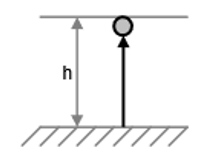
\includegraphics[width=\columnwidth]{./Images/SenkWurf.png}
	\end{minipage}%%% to prevent a space
	\begin{minipage}{0.25\textwidth}
		Fallzeit:
		\begin{formula}
			{t_f = \sqrt{\frac{2s}{g}}} 
		\end{formula}
		
		Steigzeit:
		\begin{formula}
			{t_s = \frac{v_0}{g}} 
		\end{formula}
			
		Höhe:
		\begin{formula}
			{h_{max} = \frac{v_0^2}{2g}\\
			h(t) = v_0 - \frac{g}{2}t^2}
		\end{formula}	
	\end{minipage}
\end{minipage}

\subsubsection{Horizontaler Wurf \kuchling{80}}
\begin{minipage}{\textwidth}	
	\begin{minipage}{0.2\textwidth}
		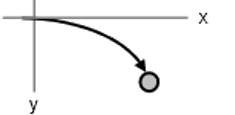
\includegraphics[width=\columnwidth]{./Images/HoriWurf.png}
	\end{minipage}%%% to prevent a space
	\begin{minipage}{0.25\textwidth}	
		x-Position:
		\begin{formula}
			{x(t) = v_0 \cdot t} 
		\end{formula}
		
		y-Position:
		\begin{formula}
			{y(t) = -\frac{g}{2}t^2}
		\end{formula}	
	\end{minipage}
\end{minipage}

\subsubsection{Schiefer Wurf \kuchling{82}}
\begin{minipage}{\textwidth}	
	\begin{minipage}{0.2\textwidth}
		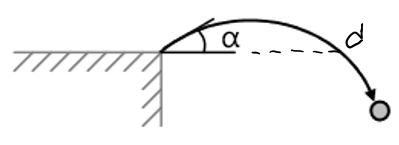
\includegraphics[width=\columnwidth]{./Images/SchiefWurf.png}
	\end{minipage}%%% to prevent a space
	\begin{minipage}{0.25\textwidth}	
		Strecke bis max Höhe:
		\begin{formula}
			{x_{maxY} = \frac{v_0^2}{g}\sin^2\alpha \cdot \cos\alpha = \frac{d}{2}} 
		\end{formula}
		
	 	Distanz
		\begin{formula}
			{d = \frac{v_0^2}{g}\cdot\sin(2\alpha)}
		\end{formula}
	
		Max Höhe:
		\begin{formula}
			{h = \frac{v_0^2}{2g}\sin^2\alpha}
		\end{formula}	
	 	
	 	Geschw.
		\begin{formula}
	 		{v_x &= v_0 \cdot \cos\alpha\\ v_y &= v_0 \cdot \sin\alpha - gt}
	 	\end{formula}	
	
	\end{minipage}
\end{minipage}

\subsection{Pendel}
\begin{minipage}{\textwidth}	
	\begin{minipage}{0.2\textwidth}
		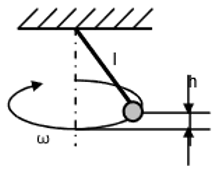
\includegraphics[width=\columnwidth]{./Images/pendel.png}
	\end{minipage}%%% to prevent a space
	\begin{minipage}{0.25\textwidth}	
		\begin{formula}
			{\omega = \sqrt{\frac{g}{l - h}}} 
		\end{formula}
	\end{minipage}
\end{minipage}
